\documentclass[UTF8,11pt,a4paper,fontset=fandol]{ctexart}
\usepackage{amsmath,amssymb,mathtools,geometry,enumitem,xcolor,hyperref,tikz,needspace}
\usetikzlibrary{arrows.meta}
\geometry{top=2.1cm,bottom=2.1cm,left=2.35cm,right=2.35cm}
\hypersetup{colorlinks=true,linkcolor=blue!45!black,pdftitle={习题三详细解答}}
\pagestyle{plain}
\setlength{\parindent}{2em}
\setlength{\parskip}{0.22em}
\setlist[enumerate,1]{label=(\arabic*),leftmargin=2.8em,itemsep=0.7em,topsep=0.35em}
\setlist[enumerate,2]{label=\arabic*.,leftmargin=2.6em,itemsep=0.4em,topsep=0.25em}
\allowdisplaybreaks[2]
\newcommand{\ii}{\mathrm{i}}
\newcommand{\ee}{\mathrm{e}}
\newcommand{\dd}{\,\mathrm{d}}
\newcommand{\Ree}{\operatorname{Re}}
\newcommand{\Imm}{\operatorname{Im}}
\newcommand{\Log}{\operatorname{Log}}
\newcommand{\idea}{\par\medskip\Needspace{3\baselineskip}\noindent\textbf{分析思路}\quad}
\newcommand{\answer}{\par\medskip\Needspace{3\baselineskip}\noindent\textbf{详细解答}\quad}
\newcommand{\method}[1]{\par\medskip\Needspace{3\baselineskip}\noindent\textbf{方法 #1}\quad}
\newcommand{\note}{\par\medskip\Needspace{3\baselineskip}\noindent\textbf{说明}\quad}
\newcommand{\problem}[1]{\par\Needspace{8\baselineskip}\section*{第 #1 题}\addcontentsline{toc}{section}{第 #1 题}}
\makeatletter
\renewcommand{\l@section}{\@dottedtocline{1}{0em}{1.5em}}
\makeatother
\title{复变函数与积分变换\\第三章习题三详细解答}
\author{}
\date{}
\begin{document}
\begin{center}
{\Large\bfseries 复变函数与积分变换\par}
\vspace{0.5em}
{\Large 第三章习题三详细解答\par}
\end{center}
\medskip
本章面向刚学完复变函数积分的同学。我们从参数化和实积分出发，逐步练习柯西积分定理、积分公式与导数估计，再讨论调和函数和共轭调和函数。每题先交代切入点，再写清计算或证明；有学习价值的不同方法一并保留。

全文除另行说明外，简单闭曲线的正向指逆时针方向。圆环区域的正向边界则是外圈逆时针、内圈顺时针。必要的条件说明均在对应题中给出，插图使用 TikZ 绘制。

{\setlength{\parskip}{0pt}\tableofcontents}
\newpage
\section*{做题前的几个提醒}
\addcontentsline{toc}{section}{做题前的几个提醒}
\begin{enumerate}
\item 参数化时不仅要替换 $z$，还要替换 $\dd z$：若 $z=z(t)$，则
\[
\int_C f(z)\dd z=\int_\alpha^\beta f(z(t))z'(t)\dd t.
\]
参数区间取 $[\alpha,\beta]$，端点和递增方向共同确定路线。
\item 若 $f=u+\ii v$，$z=x+\ii y$，也可以从
\[
f(z)\dd z=(u\dd x-v\dd y)+\ii(v\dd x+u\dd y)
\]
入手，把复积分拆成两个实曲线积分。
\item 先检查奇点位置，再选定理。本章直接使用柯西积分定理时，均检查被积函数在曲线及其内部的某个开邻域中解析。曲线上有奇点时，普通曲线积分一般没有定义，不能照套公式。
\item 柯西积分公式及高阶导数公式为
\[
\oint_C\frac{F(z)}{z-a}\dd z=2\pi\ii F(a),\qquad
\oint_C\frac{F(z)}{(z-a)^{m+1}}\dd z
=\frac{2\pi\ii}{m!}F^{(m)}(a),
\]
其中 $a$ 在正向简单闭曲线 $C$ 内，$F$ 在 $C$ 及其内部的邻域中解析。这里的阶数是“分母幂次减一”。
\end{enumerate}

\problem{1}
\textbf{题目}\quad 沿下列路线计算积分 $\displaystyle\int_0^{3+\ii}z^2\dd z$：
\begin{enumerate}
\item 自原点到 $3+\ii$ 的直线段；
\item 自原点沿实轴至 $3$，再由 $3$ 垂直向上至 $3+\ii$；
\item 自原点沿虚轴至 $\ii$，再由 $\ii$ 水平向右至 $3+\ii$。
\end{enumerate}
\idea 先按指定路线逐段参数化，借此熟悉 $\dd z$ 的处理。三条路线的起点、终点相同，而 $z^2$ 在全平面解析；算完以后还可以用原函数核验三种结果。
\answer
\begin{enumerate}
\item 直线段可写成
\[
z=(3+\ii)t,\quad 0\leqslant t\leqslant1,\quad \dd z=(3+\ii)\dd t.
\]
因此
\begin{align*}
\int_0^{3+\ii}z^2\dd z
&=(3+\ii)^3\int_0^1t^2\dd t=\frac{(3+\ii)^3}{3},\\
(3+\ii)^3&=(8+6\ii)(3+\ii)=18+26\ii.
\end{align*}
积分为 $6+\dfrac{26}{3}\ii$。
\item 第一段取 $z=x$，$0\leqslant x\leqslant3$；第二段取 $z=3+\ii y$，$0\leqslant y\leqslant1$。于是
\begin{align*}
\int_0^{3+\ii}z^2\dd z
&=\int_0^3x^2\dd x+\int_0^1(3+\ii y)^2\ii\dd y\\
&=9+\int_0^1[-6y+\ii(9-y^2)]\dd y\\
&=9-3+\ii\left(9-\frac13\right)
=6+\frac{26}{3}\ii.
\end{align*}
\item 第一段取 $z=\ii y$，$0\leqslant y\leqslant1$；第二段取 $z=x+\ii$，$0\leqslant x\leqslant3$。所以
\begin{align*}
\int_0^{3+\ii}z^2\dd z
&=\int_0^1(\ii y)^2\ii\dd y+\int_0^3(x+\ii)^2\dd x\\
&=-\frac{\ii}{3}+\int_0^3(x^2-1+2\ii x)\dd x\\
&=-\frac{\ii}{3}+(9-3)+9\ii
=6+\frac{26}{3}\ii.
\end{align*}
\end{enumerate}
\method{二：用原函数统一核验}
因为 $F(z)=z^3/3$ 是 $z^2$ 在全平面的原函数，三条路线上的积分均为
\[
F(3+\ii)-F(0)=\frac{(3+\ii)^3}{3}=6+\frac{26}{3}\ii.
\]
\note 用原函数是简洁的核验方法，但不能替代对路线参数化的练习。也不能把“端点相同就有相同积分”用于任意被积函数。

\problem{2}
\textbf{题目}\quad 分别沿 $y=x$ 与 $y=x^2$ 计算
\[
\int_0^{1+\ii}(x^2+\ii y)\dd z.
\]
\idea 被积函数含 $x,y$，先把路线条件代入。可以把 $\dd z$ 展开为 $\dd x+\ii\dd y$，也可以直接参数化 $z$。本题两条路线的结果恰好相同，但这不意味着该积分与所有路线无关。
\answer
\method{一：拆成两个实曲线积分}
由
\[
(x^2+\ii y)(\dd x+\ii\dd y)
=(x^2\dd x-y\dd y)+\ii(y\dd x+x^2\dd y),
\]
分别计算实部和虚部。
\begin{enumerate}
\item 沿 $y=x$，取 $x=t,y=t$，$0\leqslant t\leqslant1$，则
\begin{align*}
\int_0^{1+\ii}(x^2+\ii y)\dd z
&=\int_0^1(t^2-t)\dd t
+\ii\int_0^1(t+t^2)\dd t\\
&=\left(\frac13-\frac12\right)
+\ii\left(\frac12+\frac13\right)
=-\frac16+\frac56\ii.
\end{align*}
\item 沿 $y=x^2$，取 $x=t,y=t^2$，$0\leqslant t\leqslant1$，则 $\dd y=2t\dd t$，故
\begin{align*}
\int_0^{1+\ii}(x^2+\ii y)\dd z
&=\int_0^1(t^2-2t^3)\dd t
+\ii\int_0^1(t^2+2t^3)\dd t\\
&=\left(\frac13-\frac12\right)
+\ii\left(\frac13+\frac12\right)
=-\frac16+\frac56\ii.
\end{align*}
\end{enumerate}
\method{二：直接参数化复变量}
沿直线取 $z=t+\ii t$，$\dd z=(1+\ii)\dd t$；沿抛物线取 $z=t+\ii t^2$，$\dd z=(1+2\ii t)\dd t$。于是
\begin{align*}
I_{y=x}&=\int_0^1(t^2+\ii t)(1+\ii)\dd t
=-\frac16+\frac56\ii,\\
I_{y=x^2}&=\int_0^1(t^2+\ii t^2)(1+2\ii t)\dd t
=-\frac16+\frac56\ii.
\end{align*}
两个乘积展开后正是方法一的实部、虚部被积表达式。
\note 为说明结果相同只是本题两条路线的巧合，可以改走折线 $0\to1\to1+\ii$：
\[
I=\int_0^1x^2\dd x+\int_0^1(1+\ii y)\ii\dd y
=\frac13-\frac12+\ii=-\frac16+\ii,
\]
它与前两个结果不同。

\problem{3}
\textbf{题目}\quad 计算 $\displaystyle\oint_C|z|\overline z\dd z$，其中 $C$ 由直线段 $-1\leqslant x\leqslant1,y=0$ 和上半单位圆周组成。
\idea 题目未明确方向，这里取正向：实轴段从 $-1$ 到 $1$，上半圆从 $1$ 到 $-1$。两段上 $|z|$ 的表达式不同，必须分别代入。
\answer 将 $C$ 分成实轴段 $C_2$ 与上半圆弧 $C_1$，方向如下。
\begin{center}
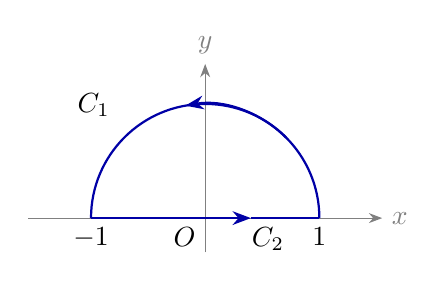
\begin{tikzpicture}[scale=1.45,>=Stealth]
\draw[->,gray] (-1.55,0)--(1.55,0) node[right]{$x$};
\draw[->,gray] (0,-.3)--(0,1.35) node[above]{$y$};
\draw[blue!65!black,thick] (1,0) arc (0:180:1);
\draw[blue!65!black,thick,->] (.707,.707) arc (45:100:1);
\draw[blue!65!black,thick,->] (-1,0)--(.4,0);
\draw[blue!65!black,thick] (.4,0)--(1,0);
\node[below] at (-1,0){$-1$}; \node[below] at (1,0){$1$};
\node[below left] at (0,0){$O$};
\node[above left] at (-.75,.8){$C_1$}; \node[below] at (.55,0){$C_2$};
\end{tikzpicture}
\end{center}
在 $C_1$ 上取 $z=\ee^{\ii\theta}$，$0\leqslant\theta\leqslant\pi$。于是 $|z|=1$，$\overline z=\ee^{-\ii\theta}$，
\[
\int_{C_1}|z|\overline z\dd z
=\int_0^\pi\ee^{-\ii\theta}\ii\ee^{\ii\theta}\dd\theta
=\pi\ii.
\]
在 $C_2$ 上取 $z=x$，$-1\leqslant x\leqslant1$，则
\[
\int_{C_2}|z|\overline z\dd z
=\int_{-1}^1|x|x\dd x
=-\int_{-1}^0x^2\dd x+\int_0^1x^2\dd x=0.
\]
两段相加，所求积分为 $\pi\ii$。若取相反方向，则结果为 $-\pi\ii$。

\problem{4}
\textbf{题目}\quad 证明：
\begin{enumerate}
\item $\displaystyle\left|\int_C(x^2+\ii y^2)\dd z\right|\leqslant2$，$C$ 为从 $-\ii$ 到 $\ii$ 的直线段；
\item $\displaystyle\left|\int_C(x^2+\ii y^2)\dd z\right|\leqslant\pi$，$C$ 为从 $-\ii$ 到 $\ii$ 的右半单位圆周。
\end{enumerate}
\idea 证明上界时，通常不必先求积分的准确值。使用估值不等式
\[
\left|\int_C f(z)\dd z\right|\leqslant\int_C|f(z)|\dd s\leqslant ML,
\]
其中 $M$ 是曲线上 $|f|$ 的上界，$L$ 是曲线长度。还可以直接计算积分，作为另一种验证。
\answer
\method{一：估值不等式}
\begin{enumerate}
\item 直线段上 $x=0$、$-1\leqslant y\leqslant1$，所以
\[
|x^2+\ii y^2|=y^2\leqslant1.
\]
线段长为 $2$，故积分的模不超过 $1\times2=2$。
\item 右半单位圆上 $x^2+y^2=1$，$|x|,|y|\leqslant1$。因而
\[
|x^2+\ii y^2|=\sqrt{x^4+y^4}
\leqslant\sqrt{x^2+y^2}=1.
\]
半圆弧长为 $\pi$，故积分的模不超过 $\pi$。
\end{enumerate}
\method{二：直接计算并比较}
\begin{enumerate}
\item 取 $z=\ii y$，$-1\leqslant y\leqslant1$，则
\[
\int_C(x^2+\ii y^2)\dd z=-\int_{-1}^1y^2\dd y=-\frac23.
\]
其模为 $2/3<2$。
\item 取 $z=\ee^{\ii\theta}$，$-\pi/2\leqslant\theta\leqslant\pi/2$。代入 $x=\cos\theta,y=\sin\theta$ 后，
\begin{align*}
(x^2+\ii y^2)\dd z
={}&[-\cos^2\theta\sin\theta-\sin^2\theta\cos\theta]\dd\theta\\
&+\ii[\cos^3\theta-\sin^3\theta]\dd\theta.
\end{align*}
对称区间上两个奇函数的积分为零，而
\[
\int_{-\pi/2}^{\pi/2}\sin^2\theta\cos\theta\dd\theta
=\int_{-1}^1s^2\dd s=\frac23,
\]
\[
\int_{-\pi/2}^{\pi/2}\cos^3\theta\dd\theta
=\int_{-1}^1(1-s^2)\dd s=\frac43.
\]
所以积分为 $-\dfrac23+\dfrac43\ii$，其模为
\[
\frac{2\sqrt5}{3}<2<\pi.
\]
\end{enumerate}
\note 方法一更直接回应“证明不等式”的要求；方法二同时得到准确值，可用来核验估计。

\problem{5}
\textbf{题目}\quad 设 $f$ 在单连通区域 $D$ 内解析，$C$ 为 $D$ 内任意正向简单闭曲线。问
\[
\oint_C\Ree[f(z)]\dd z=\oint_C\Imm[f(z)]\dd z=0
\]
是否成立？成立则证明，不成立则举例。
\idea 柯西积分定理适用于解析的被积函数。$f$ 解析不表示 $\Ree f$ 和 $\Imm f$ 作为复变量函数也解析。取最简单的 $f(z)=z$、单位圆即可检验。
\answer 不成立。取 $D=\mathbb C$，$f(z)=z$，$C:|z|=1$ 正向。令 $z=\ee^{\ii\theta}$，$0\leqslant\theta\leqslant2\pi$，则
\begin{align*}
\oint_C\Ree z\dd z
&=\int_0^{2\pi}\cos\theta\,\ii\ee^{\ii\theta}\dd\theta\\
&=-\int_0^{2\pi}\cos\theta\sin\theta\dd\theta
+\ii\int_0^{2\pi}\cos^2\theta\dd\theta=\pi\ii,\\
\oint_C\Imm z\dd z
&=\int_0^{2\pi}\sin\theta\,\ii\ee^{\ii\theta}\dd\theta\\
&=-\int_0^{2\pi}\sin^2\theta\dd\theta
+\ii\int_0^{2\pi}\sin\theta\cos\theta\dd\theta=-\pi.
\end{align*}
两个积分均不为零，已经否定原断言。
\note $\oint_C f(z)\dd z=0$ 只能推出
\[
\oint_C\Ree f\dd z+\ii\oint_C\Imm f\dd z=0,
\]
这里两个积分本身都是复数，不能把它们误当成 $\oint_C f\dd z$ 的实部、虚部。本例正是 $\pi\ii+\ii(-\pi)=0$。

\problem{6}
\textbf{题目}\quad 利用单位圆上 $\overline z=1/z$ 的性质及柯西积分公式说明
\[
\oint_C\overline z\dd z=2\pi\ii,
\]
其中 $C$ 为正向单位圆周。
\idea 虽然 $\overline z$ 不解析，但积分只用到曲线上的函数值。可以在单位圆上把它换成 $1/z$，再对常函数 $F(z)=1$ 使用积分公式。
\answer
\method{一：按题意使用柯西积分公式}
在 $C$ 上 $z\overline z=|z|^2=1$，所以
\[
\oint_C\overline z\dd z
=\oint_C\frac1z\dd z=2\pi\ii F(0)=2\pi\ii,
\quad F\equiv1.
\]
\method{二：参数化核验}
取 $z=\ee^{\ii\theta}$，$0\leqslant\theta\leqslant2\pi$，则
\[
\oint_C\overline z\dd z
=\int_0^{2\pi}\ee^{-\ii\theta}\ii\ee^{\ii\theta}\dd\theta
=2\pi\ii.
\]
\note $\overline z=1/z$ 只在本题的单位圆上成立，不是其内部的函数恒等式。

\problem{7}
\textbf{题目}\quad 计算 $\displaystyle\oint_C\frac{\overline z}{|z|}\dd z$，$C$ 分别为正向圆周 (1) $|z|=2$；(2) $|z|=4$。
\idea 两种圆周只差半径，先对 $|z|=r>0$ 求一个统一公式。可以在圆周上化简被积函数，也可以直接参数化。
\answer
\method{一：在圆周上化为柯西积分公式}
由 $z\overline z=|z|^2$，在 $|z|=r$ 上有
\[
\frac{\overline z}{|z|}=\frac{|z|}{z}=\frac rz.
\]
所以
\[
\oint_C\frac{\overline z}{|z|}\dd z
=r\oint_C\frac1z\dd z=2\pi r\ii.
\]
\method{二：参数化圆周}
取 $z=r\ee^{\ii\theta}$，$0\leqslant\theta\leqslant2\pi$。则
\[
\frac{\overline z}{|z|}=\ee^{-\ii\theta},\qquad
\dd z=\ii r\ee^{\ii\theta}\dd\theta,
\]
从而积分为 $\int_0^{2\pi}\ii r\dd\theta=2\pi r\ii$。
代入 $r=2,4$，分别得到 $4\pi\ii$ 和 $8\pi\ii$。

\problem{8}
\textbf{题目}\quad 直接给出下列积分的结果，并说明理由：
\begin{enumerate}
\item $\displaystyle\oint_{|z|=1}\frac{3z+5}{z^2+2z+4}\dd z$；
\item $\displaystyle\oint_{|z|=1}\frac{\ee^z}{\cos z}\dd z$；
\item $\displaystyle\oint_{|z|=2}\ee^z(z^2+1)\dd z$；
\item $\displaystyle\oint_{|z|=1/2}\frac{\dd z}{(z^2-1)(z^3-1)}$。
\end{enumerate}
\idea 本题的关键不是计算，而是确认被积函数在圆周及其内部的邻域中解析。有分母时先列出分母的全部零点。
\answer
\begin{enumerate}
\item $z^2+2z+4=0$ 的根为 $-1\pm\sqrt3\ii$，模均为 $2>1$。因此被积函数在闭单位圆盘的邻域中解析，积分为 $0$。
\item 由 $\cos z=(\ee^{\ii z}+\ee^{-\ii z})/2$，$\cos z=0$ 等价于 $\ee^{2\ii z}=-1$。写 $z=x+\ii y$，比较模得 $\ee^{-2y}=1$，故 $y=0$；再比较角度得
\[
z=\frac\pi2+k\pi,\qquad k\in\mathbb Z.
\]
这些点的模至少为 $\pi/2>1$，故被积函数在闭单位圆盘的邻域中解析，积分为 $0$。
\item $\ee^z(z^2+1)$ 在全平面解析，积分为 $0$。
\item 分母零点为
\[
1,\ -1,\ -\frac12+\frac{\sqrt3}{2}\ii,\ -\frac12-\frac{\sqrt3}{2}\ii,
\]
模均为 $1>1/2$。因此被积函数在 $|z|\leqslant1/2$ 的邻域中解析，积分为 $0$。
\end{enumerate}
\note 四小题都使用柯西积分定理：确认曲线及其内部没有奇点后，积分直接为零。

\problem{9}
\textbf{题目}\quad 沿指定曲线的正向计算下列积分：
\begin{enumerate}[itemsep=0.3em]
\item $\displaystyle\oint_C\frac{\ee^z}{z-2}\dd z$，$C:|z-2|=1$；
\item $\displaystyle\oint_C\frac{\cos\pi z}{(z-1)^5}\dd z$，$C:|z|=r>1$；
\item $\displaystyle\oint_C\frac{\sin z}{(z-\pi/2)^2}\dd z$，$C:|z|=2$；
\item $\displaystyle\oint_C\frac{\dd z}{(z^2+1)(z^2+4)}$，$C:|z|=3/2$；
\item $\displaystyle\oint_C\frac{3z^2+7z+1}{(z+1)^3}\dd z$，$C:|z+\ii|=1$；
\item $\displaystyle\oint_C\frac{\dd z}{z^2-a^2}$，$C:|z-a|=a$，$a>0$；
\item $\displaystyle\oint_C\frac{\cos z}{z^3}\dd z$，$C=C_1+C_2$，$C_1:|z|=2$，$C_2:|z|=3$；
\item $\displaystyle\oint_C\frac{\ee^z}{(z-a)^3}\dd z$，$|a|\ne1$，$C:|z|=1$；
\item $\displaystyle\oint_C\frac{\ee^z\sin z}{z^2}\dd z$，$C:|z-\ii|=2$；
\item $\displaystyle\oint_C\frac{3z+2}{z^4-1}\dd z$，$C:|z-(1+\ii)|=\sqrt2$。
\end{enumerate}
\idea 每次按“找奇点---判位置---选公式---算导数”的顺序做。多个内部奇点时，不能把含有另一个内部奇点的函数直接当作积分公式中的解析分子；可先作部分分式分解，或变形到各奇点附近的小圆。
\answer
\begin{enumerate}
\item 唯一奇点 $2$ 位于圆心，$F(z)=\ee^z$ 在全平面解析。由积分公式，
\[
I=2\pi\ii F(2)=2\pi\ii\ee^2.
\]
\item $1$ 在 $|z|=r>1$ 内。分母为五次幂，需取四阶导数。逐次求导为
\[
F'=-\pi\sin\pi z,\quad F''=-\pi^2\cos\pi z,
\]
\[
F'''=\pi^3\sin\pi z,\quad F^{(4)}=\pi^4\cos\pi z.
\]
因此 $F^{(4)}(1)=-\pi^4$，
\[
I=\frac{2\pi\ii}{4!}(-\pi^4)=-\frac{\pi^5}{12}\ii.
\]
\item $\pi/2<2$，奇点在圆内。取 $F(z)=\sin z$，需计算一阶导数，故
\[
I=2\pi\ii F'(\pi/2)=2\pi\ii\cos(\pi/2)=0.
\]
注意结果为零不是因为被积函数在圆内解析，而是公式中的导数值为零。
\item 奇点为 $\pm\ii,\pm2\ii$；只有 $\pm\ii$ 在 $|z|<3/2$ 内。
\method{一：变形到两个小圆}
先分解
\[
\frac1{(z^2+1)(z^2+4)}
=\frac13\left(\frac1{z^2+1}-\frac1{z^2+4}\right).
\]
第二项在闭圆盘的邻域中解析，闭路积分为零。对第一项，在 $\ii$ 和 $-\ii$ 附近各取正向小圆 $\gamma_+$、$\gamma_-$，使它们互不相交且在 $C$ 内。被积函数在去掉这两个小圆盘后的区域中解析，由多连通区域的柯西积分定理，
\[
\oint_C\frac{\dd z}{z^2+1}
=\oint_{\gamma_+}\frac{\dd z}{(z-\ii)(z+\ii)}
+\oint_{\gamma_-}\frac{\dd z}{(z-\ii)(z+\ii)}.
\]
分别使用积分公式得到
\[
\oint_{\gamma_+}\frac{\dd z}{z^2+1}
=2\pi\ii\frac1{2\ii}=\pi,
\qquad
\oint_{\gamma_-}\frac{\dd z}{z^2+1}
=2\pi\ii\frac1{-2\ii}=-\pi.
\]
两项抵消，故原积分 $I=0$。
\method{二：完全化为简单分式}
由
\[
\frac1{z^2+1}=\frac1{2\ii}\left(\frac1{z-\ii}-\frac1{z+\ii}\right),
\]
两项在 $C$ 内分别含一个奇点，积分均为 $2\pi\ii$。故
\[
I=\frac1{6\ii}(2\pi\ii-2\pi\ii)-\frac13\cdot0=0.
\]
两种方法表达的是同一件事：内部两个奇点的贡献恰好相消。
\item 唯一奇点为 $-1$。它到圆心 $-\ii$ 的距离是
\[
|-1+\ii|=\sqrt2>1,
\]
所以它在圆外。被积函数在闭圆盘的邻域中解析，$I=0$。不要看到三次幂就不检查位置地套高阶导数公式。
\item 因式分解 $z^2-a^2=(z-a)(z+a)$。$a$ 在圆心，$-a$ 到圆心的距离为 $2a>a$，故 $-a$ 在圆外。于是 $F(z)=1/(z+a)$ 在闭圆盘的邻域中解析，
\[
I=\oint_C\frac{F(z)}{z-a}\dd z
=2\pi\ii F(a)=\frac{\pi\ii}{a}.
\]
也可以作部分分式分解
\[
\frac1{z^2-a^2}=\frac1{2a}\left(\frac1{z-a}-\frac1{z+a}\right),
\]
两个积分分别为 $2\pi\ii$ 和 $0$，结果相同。
\item \textbf{本小题需先说明方向。}若按题首“各曲线正向”理解，$C_1,C_2$ 均逆时针；若把 $C$ 看作圆环的正向边界，则 $C_1$ 应顺时针、$C_2$ 逆时针。这两种解释的答案不同。

先记 $J_R$ 为 $|z|=R$ 逆时针方向的积分。原点在圆内，$F(z)=\cos z$，$F''(0)=-1$，故
\[
J_R=\frac{2\pi\ii}{2!}F''(0)=-\pi\ii\quad(R>0).
\]
\begin{itemize}
\item 若两圈均逆时针，则 $I=J_2+J_3=-2\pi\ii$。
\item 若 $C$ 为圆环 $2<|z|<3$ 的正向边界，则 $I=J_3-J_2=0$。
\end{itemize}
第二种约定也可以直接由柯西积分定理得到：$\cos z/z^3$ 在圆环及其边界的邻域中解析，外圈积分减去内圈逆时针积分为零。这不表示每个单独的圆周积分都为零。
\begin{center}
\begin{tikzpicture}[scale=.67,>=Stealth]
\fill[blue!6,even odd rule] (0,0) circle (3) (0,0) circle (2);
\draw[->,gray] (-3.5,0)--(3.5,0) node[right]{$x$};
\draw[->,gray] (0,-3.4)--(0,3.5) node[above]{$y$};
\draw[blue!65!black,thick] (0,0) circle (3);
\draw[blue!65!black,thick] (0,0) circle (2);
\draw[blue!65!black,thick,->] (3,0) arc (0:40:3);
\draw[blue!65!black,thick,->] (2,0) arc (0:-55:2);
\draw[fill=white] (0,0) circle (.06); \node[below left] at (0,0){$O$};
\node[above right] at (2.2,2.2){$C_2$};
\node[above right] at (1.35,1.35){$C_1$};
\node at (0,-4){圆环正向边界：外圈逆时针，内圈顺时针};
\end{tikzpicture}
\end{center}
\item 唯一奇点为 $a$，按它与单位圆的位置分类：
\[
I=\begin{cases}
\dfrac{2\pi\ii}{2!}(\ee^z)''\big|_{z=a}=\pi\ii\ee^a,&|a|<1,\\[4pt]
0,&|a|>1.
\end{cases}
\]
后一种情形使用柯西积分定理；$|a|=1$ 被排除，是为了避免曲线上有奇点。
\item 原点到圆心 $\ii$ 的距离为 $1<2$，故原点在圆内。取 $F(z)=\ee^z\sin z$，则
\[
F'(z)=\ee^z(\sin z+\cos z),\qquad F'(0)=1.
\]
于是 $I=2\pi\ii F'(0)=2\pi\ii$。
\item 分母的零点为 $1,-1,\ii,-\ii$。到圆心 $1+\ii$ 的距离分别是
\[
1,\quad\sqrt5,\quad1,\quad\sqrt5.
\]
因此只有 $1,\ii$ 在圆内，没有奇点在圆周上。
\begin{center}
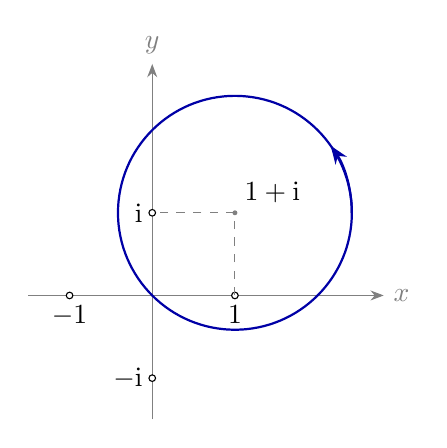
\begin{tikzpicture}[scale=1.05,>=Stealth]
\draw[->,gray] (-1.5,0)--(2.8,0) node[right]{$x$};
\draw[->,gray] (0,-1.5)--(0,2.8) node[above]{$y$};
\draw[blue!65!black,thick] (1,1) circle ({sqrt(2)});
\draw[blue!65!black,thick,->] ({1+sqrt(2)},1) arc (0:35:{sqrt(2)});
\foreach \x/\y/\lab/\pos in {1/0/1/below,-1/0/-1/below,0/1/\ii/left,0/-1/-\ii/left}{
\draw[fill=white] (\x,\y) circle (.04); \node[\pos] at (\x,\y){$\lab$};}
\draw[gray,dashed] (1,0)--(1,1)--(0,1);
\fill[gray] (1,1) circle (.03); \node[above right] at (1,1){$1+\ii$};
\end{tikzpicture}
\end{center}
图中的实线是积分路径；空心点标示被积函数的奇点，这些点不属于函数定义域。
\method{一：直接裂项}
令
\[
H(z)=\frac{3z+2}{(z+1)(z+\ii)}.
\]
$H$ 的两个奇点均在 $C$ 外，因此 $H$ 在 $C$ 及其内部的邻域中解析。由
\[
\frac1{(z-1)(z-\ii)}
=\frac1{1-\ii}\left(\frac1{z-1}-\frac1{z-\ii}\right),
\]
得到
\begin{align*}
I&=\frac1{1-\ii}\left[\oint_C\frac{H(z)}{z-1}\dd z
-\oint_C\frac{H(z)}{z-\ii}\dd z\right]\\
&=\frac{2\pi\ii}{1-\ii}[H(1)-H(\ii)].
\end{align*}
逐项算出
\[
H(1)=\frac5{2(1+\ii)}=\frac{5-5\ii}{4},\qquad
H(\ii)=\frac{2+3\ii}{(1+\ii)2\ii}=\frac{1-5\ii}{4}.
\]
两者相减为 $1$，所以
\[
I=\frac{2\pi\ii}{1-\ii}=\pi(-1+\ii).
\]
\method{二：变形到两个小圆}
在 $1,\ii$ 附近取互不相交的正向小圆 $\gamma_1,\gamma_\ii$，并均置于 $C$ 内。由多连通区域的积分定理，原积分等于两个小圆上的积分之和。分别记这两个积分为 $I_1,I_\ii$，在每个小圆上使用积分公式，得到
\begin{align*}
I_1&=2\pi\ii\frac{3z+2}{(z+1)(z+\ii)(z-\ii)}\bigg|_{z=1}
=2\pi\ii\cdot\frac54,\\
I_\ii&=2\pi\ii\frac{3z+2}{(z+1)(z+\ii)(z-1)}\bigg|_{z=\ii}
=2\pi\ii\left(-\frac34+\frac\ii2\right).
\end{align*}
所以
\[
I=I_1+I_\ii=2\pi\ii\left(\frac54-\frac34+\frac\ii2\right)
=\pi(-1+\ii).
\]
这正好说明两个内部奇点的贡献怎样相加，不需要预先使用第五章的留数定理。
\end{enumerate}
\note 第 (4)、(10) 小题的“小圆变形”有共同依据：去掉小圆盘后应用柯西积分定理。该区域的内边界为顺时针方向；移项以后，小圆积分统一写成逆时针的正向积分。第 (7) 小题的方向歧义必须保留说明，不能在未说明方向时只给一个数值。

\problem{10}
\textbf{题目}\quad 设 $C$ 为不经过 $a,-a$ 的正向简单闭曲线，$a\ne0$。按 $a,-a$ 与 $C$ 的不同位置，计算
\[
\oint_C\frac{z}{z^2-a^2}\dd z.
\]
\idea 两个分母因子不同，先分解为简单分式。每个内部奇点贡献 $\pi\ii$，外部奇点贡献零。也可以用两个小圆分拆积分，理解多个奇点的处理。
\answer
\method{一：直接裂项}
有
\[
\frac{z}{z^2-a^2}
=\frac12\left(\frac1{z-a}+\frac1{z+a}\right).
\]
由柯西积分公式和积分定理，
\[
\oint_C\frac{\dd z}{z-b}
=\begin{cases}2\pi\ii,&b\text{ 在 }C\text{ 内},\\0,&b\text{ 在 }C\text{ 外}.
\end{cases}
\]
因此
\[
\oint_C\frac{z}{z^2-a^2}\dd z
=\begin{cases}
0,&a,-a\text{ 均在 }C\text{ 外},\\
\pi\ii,&a,-a\text{ 恰有一个在 }C\text{ 内},\\
2\pi\ii,&a,-a\text{ 均在 }C\text{ 内}.
\end{cases}
\]
\method{二：小圆变形法}
若两个点都在 $C$ 内，取足够小的正向圆周 $\gamma_a:|z-a|=\varepsilon$ 和 $\gamma_{-a}:|z+a|=\varepsilon$，使其互不相交且在 $C$ 内。按第 9 题说明的变形原理，原积分等于两个小圆积分之和。
在 $\gamma_a$ 内 $1/(z+a)$ 解析，所以
\[
\oint_{\gamma_a}\frac{z}{z^2-a^2}\dd z
=\frac12\left(2\pi\ii+0\right)=\pi\ii.
\]
同理在 $\gamma_{-a}$ 内 $1/(z-a)$ 解析，另一个小圆积分也为 $\pi\ii$，相加为 $2\pi\ii$。
若只有一个点在内部，只保留对应小圆，积分为 $\pi\ii$；若两个点都在外部，被积函数在 $C$ 及其内部的邻域中解析，积分为零。
\note 本题 $a$ 可以是任意非零复数，而不只是正实数。$a\ne0$ 保证两个奇点不同，“$C$ 不经过 $\pm a$”保证积分路径上没有奇点。

\problem{11}
\textbf{题目}\quad $f,g$ 在区域 $D$ 内解析，$C$ 为 $D$ 内一条简单光滑闭曲线，且内部全属于 $D$。若 $f=g$ 在 $C$ 上处处成立，证明 $f=g$ 在 $C$ 内处处成立。
\idea 内部每一点的函数值都可以用边界上的值通过柯西积分公式表示。边界值相同，内部值便相同。积分中的变量用 $\zeta$，避免与待求值的点 $z$ 混淆。
\answer 不妨把 $C$ 取为正向；固定其内部任意一点 $z$。因为 $f,g$ 在 $C$ 及其内部的邻域中解析，积分公式给出
\[
f(z)=\frac1{2\pi\ii}\oint_C\frac{f(\zeta)}{\zeta-z}\dd\zeta,
\qquad
g(z)=\frac1{2\pi\ii}\oint_C\frac{g(\zeta)}{\zeta-z}\dd\zeta.
\]
相减并使用边界条件 $f(\zeta)-g(\zeta)=0$，得到
\[
f(z)-g(z)=\frac1{2\pi\ii}\oint_C
\frac{f(\zeta)-g(\zeta)}{\zeta-z}\dd\zeta=0.
\]
由于 $z$ 是任意内部点，结论成立。
\note 条件“内部全属于 $D$”使积分公式可以使用。这里只需证明 $C$ 内部的结论，无须扩展到整个 $D$。

\problem{12}
\textbf{题目}\quad 验证下列函数是调和函数，并求出以 $z=x+\ii y$ 为自变量的解析函数 $f(z)=u+\ii v$：
\begin{enumerate}
\item $v=\arctan(y/x)$，$x>0$；
\item $u=\ee^x(y\cos y+x\sin y)+x+y$，$f(0)=\ii$；
\item $u=(x-y)(x^2+4xy+y^2)$；
\item $v=y/(x^2+y^2)$，$f(2)=0$。
\end{enumerate}
\idea “调和”只检查 $u_{xx}+u_{yy}=0$ 或 $v_{xx}+v_{yy}=0$；“构造解析函数”还要让两分量配对满足 C--R 方程
\[
u_x=v_y,\qquad u_y=-v_x.
\]
若已知 $u$，先由 $v_y=u_x$ 积分，再用 $v_x=-u_y$ 确定只依赖 $x$ 的积分函数；已知 $v$ 时反过来做。最后才把答案识别为 $z$ 的函数，并使用给定函数值确定常数。
\answer
\begin{enumerate}
\item \textbf{验证调和性。}在右半平面 $x>0$ 上，
\[
v_x=-\frac{y}{x^2+y^2},\qquad v_y=\frac{x}{x^2+y^2},
\]
\[
v_{xx}=\frac{2xy}{(x^2+y^2)^2},\qquad
v_{yy}=-\frac{2xy}{(x^2+y^2)^2}.
\]
它们连续且和为零，故 $v$ 调和。

\textbf{求与 $v$ 配对的实部。}由 $u_x=v_y$，在 $y$ 固定时对 $x$ 积分，得
\[
u=\frac12\ln(x^2+y^2)+\varphi(y).
\]
再对 $y$ 求导，并与 $-v_x$ 比较，
\[
u_y=\frac{y}{x^2+y^2}+\varphi'(y)
=-v_x=\frac{y}{x^2+y^2},
\]
故 $\varphi'(y)=0$，$\varphi(y)=c$，$c\in\mathbb R$。因此
\[
f(z)=\frac12\ln(x^2+y^2)+c+\ii\arctan\frac yx.
\]
在右半平面上取 $\Log z=\ln|z|+\ii\arctan(y/x)$，它是解析的对数分支。于是
\[
f(z)=\Log z+c,\qquad \Ree z>0,\quad c\in\mathbb R.
\]
\note 题目给定了虚部，所以实部可以相差一个实常数 $c$；不能再任意添加虚常数，否则会改变给定的 $v$。

\item \textbf{验证调和性。}直接计算：
\begin{align*}
u_x&=\ee^x[y\cos y+(x+1)\sin y]+1,\\
u_y&=\ee^x[(x+1)\cos y-y\sin y]+1,\\
u_{xx}&=\ee^x[y\cos y+(x+2)\sin y],\\
u_{yy}&=-\ee^x[y\cos y+(x+2)\sin y].
\end{align*}
因此 $u_{xx}+u_{yy}=0$，$u$ 在全平面调和。

\method{一：由 C--R 方程求共轭调和函数}
由 $v_y=u_x$，注意
\[
\int y\cos y\dd y=y\sin y+\cos y,\qquad
\int(x+1)\sin y\dd y=-(x+1)\cos y,
\]
其中对 $y$ 积分时 $x$ 是常数。所以
\[
v=\ee^x(y\sin y-x\cos y)+y+\varphi(x).
\]
再求 $x$ 偏导：
\[
v_x=\ee^x[y\sin y-(x+1)\cos y]+\varphi'(x).
\]
与 $-u_y$ 比较，得 $\varphi'(x)=-1$，故 $\varphi(x)=-x+c$。由 $u(0,0)=0$ 和 $f(0)=\ii$，知 $v(0,0)=1$，所以 $c=1$。
\[
v=\ee^x(y\sin y-x\cos y)+y-x+1.
\]
为把答案化为 $z$ 的形式，展开
\[
z\ee^z=\ee^x[(x\cos y-y\sin y)+\ii(x\sin y+y\cos y)].
\]
其虚部正是 $u$ 中的指数项，因此 $-\ii z\ee^z$ 的实部等于该项；同时 $(1-\ii)z$ 的实部为 $x+y$。最终
\[
f(z)=-\ii z\ee^z+(1-\ii)z+\ii.
\]
\method{二：从熟悉的解析函数识别实部}
由上述展开可直接看出
\[
\Ree[-\ii z\ee^z+(1-\ii)z]=u.
\]
故 $f=-\ii z\ee^z+(1-\ii)z+\ii c$ 是所求函数族；代入 $z=0$ 得 $c=1$。方法二短一些，但方法一更能练习如何确定积分函数。

\item 先展开
\[
u=x^3+3x^2y-3xy^2-y^3.
\]
一、二阶偏导分别为
\[
u_x=3x^2+6xy-3y^2,\qquad
u_y=3x^2-6xy-3y^2,
\]
\[
u_{xx}=6x+6y,\qquad u_{yy}=-6x-6y.
\]
所以 $u$ 在全平面调和。
由 $v_y=u_x$ 积分得到
\[
v=3x^2y+3xy^2-y^3+\varphi(x).
\]
再由 $v_x=-u_y$，
\[
6xy+3y^2+\varphi'(x)=-3x^2+6xy+3y^2,
\]
得 $\varphi'(x)=-3x^2$，故 $\varphi(x)=-x^3+c$。于是
\[
v=-x^3+3x^2y+3xy^2-y^3+c.
\]
由
\[
z^3=(x^3-3xy^2)+\ii(3x^2y-y^3),
\]
可识别出
\[
f(z)=(1-\ii)z^3+\ii c,\qquad c\in\mathbb R.
\]
没有给定函数值时，虚部中的实常数 $c$ 应保留。

\item 函数的自然定义域是 $z\ne0$。为简化式子，记 $s=x^2+y^2$。有
\[
v_x=-\frac{2xy}{s^2},\qquad v_y=\frac{x^2-y^2}{s^2},
\]
\[
v_{xx}=\frac{6x^2y-2y^3}{s^3},\qquad
v_{yy}=\frac{2y^3-6x^2y}{s^3}.
\]
因此 $v_{xx}+v_{yy}=0$，且这些偏导在 $s>0$ 时连续，故 $v$ 在去掉原点的平面内调和。

由 $u_x=v_y$，观察到
\[
\frac{\partial}{\partial x}\left(-\frac x{x^2+y^2}\right)
=\frac{x^2-y^2}{(x^2+y^2)^2},
\]
所以可取
\[
u=-\frac{x}{x^2+y^2}+c.
\]
此时 $u_y=2xy/s^2=-v_x$，两条 C--R 方程都成立。与此 $v$ 配对的实部在连通定义域中只差一个实常数。由 $f(2)=0$，$v(2,0)=0$，而 $u(2,0)=-1/2+c$，故 $c=1/2$。
\[
f(z)=-\frac{x}{x^2+y^2}+\frac12
+\ii\frac{y}{x^2+y^2}
=-\frac1z+\frac12,\qquad z\ne0.
\]
\note 本小题的去心平面并非单连通区域，但上面已构造出全域单值的解析函数，所以本例可以全域配对。不能反过来认为任意多连通区域中的调和函数都有全域共轭调和函数。
\end{enumerate}

\problem{13}
\textbf{题目}\quad 设 $u$ 为区域 $D$ 中的调和函数，问
\[
f(z)=u_x-\ii u_y
\]
是否在 $D$ 中解析，为什么？
\idea 设 $a=u_x$、$b=-u_y$。检查 $a_x=b_y$ 要用调和方程，检查 $a_y=-b_x$ 要用混合偏导相等。还要说明这些一阶偏导连续，才能引用 C--R 方程的充分条件。
\answer 是解析函数。按调和函数的定义，$u$ 具有连续的二阶偏导，并满足
\[
u_{xx}+u_{yy}=0.
\]
记 $f=a+\ii b$，其中 $a=u_x,b=-u_y$。则
\[
a_x=u_{xx}=-u_{yy}=b_y,
\]
又由二阶偏导连续，$u_{xy}=u_{yx}$，故
\[
a_y=u_{xy}=u_{yx}=-b_x.
\]
$a,b$ 的一阶偏导均连续，并在 $D$ 内处处满足 C--R 方程，故 $f$ 在 $D$ 内解析。
\note 本题不要求 $D$ 单连通，也不需要先构造 $u$ 的全域共轭调和函数。若局部有解析函数 $F=u+\ii v$，则 $F'=u_x-\ii u_y$，这也解释了本题函数的形式。

\problem{14}
\textbf{题目}\quad $v=x+y$ 是 $u=x+y$ 的共轭调和函数吗？为什么？
\idea “两个函数分别调和”与“二者构成共轭调和函数”是不同条件。后者要求按 $u+\ii v$ 的次序满足 C--R 方程。
\answer 不是。虽然两函数的二阶偏导都为零，因此各自调和，但
\[
u_x=1=v_y,\qquad u_y=1\ne-v_x=-1.
\]
第二条 C--R 方程不成立，故 $v$ 不是 $u$ 的共轭调和函数。
\note 若要为 $u=x+y$ 找共轭调和函数，可由 $v_y=1$、$v_x=-1$ 得
\[
v=y-x+c,\qquad f(z)=(1-\ii)z+\ii c.
\]
这与第 12（2）题线性项的配对完全一致。

\problem{15}
\textbf{题目}\quad 若 $f(z)=u+\ii v$ 解析，证明：
\begin{enumerate}
\item $\overline{\ii\,\overline{f(z)}}$ 也解析；
\item $-u$ 是 $v$ 的共轭调和函数。
\end{enumerate}
\idea 第 (1) 小题先化简双重共轭，写出新函数的实部和虚部，再用原函数的 C--R 方程验证新函数也满足 C--R 方程。第 (2) 小题则由新函数的实部、虚部直接得到。
\answer
\begin{enumerate}
\item 利用共轭与乘法的关系及双重共轭，
\[
\overline{\ii\,\overline{f(z)}}
=\overline\ii\;\overline{\overline{f(z)}}=-\ii f(z)=v-\ii u.
\]
因为 $f=u+\ii v$ 解析，所以 $u,v$ 的一阶偏导连续，且满足
\[
u_x=v_y,\qquad u_y=-v_x.
\]
先由第一式得到
\[
v_y=u_x=-(-u)_x,
\]
再由第二式得到
\[
v_x=-u_y=(-u)_y.
\]
把新函数的实部记为 $U=v$、虚部记为 $V=-u$，上面两式正是
\[
U_x=V_y,\qquad U_y=-V_x.
\]
$U,V$ 的一阶偏导也连续，因此由 C--R 方程的充分条件，$v-\ii u=\overline{\ii\,\overline{f(z)}}$ 是解析函数。
\item 第 (1) 小题已证明 $v+\ii(-u)$ 解析。它的实部是 $v$，虚部是 $-u$，按共轭调和函数的定义，$-u$ 就是 $v$ 的共轭调和函数。
\end{enumerate}
\note 这里的次序和负号不能省略：$v$ 是 $u$ 的共轭调和函数时，一般不是 $u$、而是 $-u$，成为 $v$ 的共轭调和函数。

\problem{16}
\textbf{题目}\quad 证明 $u=x^2-y^2$ 与 $v=y/(x^2+y^2)$ 都是调和函数，但 $u+\ii v$ 不是解析函数。
\idea 分别检查两函数是否满足拉普拉斯方程，再检查它们的一阶偏导是否满足 C--R 方程。各自调和不表示它们能配成解析函数。
\answer 对 $u$，
\[
u_{xx}=2,\qquad u_{yy}=-2,
\]
故 $u$ 在全平面调和。对 $v$，第 12（4）题已算得
\[
v_{xx}=\frac{6x^2y-2y^3}{(x^2+y^2)^3},\qquad
v_{yy}=-v_{xx},
\]
故 $v$ 在 $z\ne0$ 的区域中调和。

但它们的一阶偏导为
\[
u_x=2x,\quad u_y=-2y,\quad
v_x=-\frac{2xy}{(x^2+y^2)^2},\quad
v_y=\frac{x^2-y^2}{(x^2+y^2)^2}.
\]
C--R 方程 $u_x=v_y$、$u_y=-v_x$ 并不恒成立。例如在 $(1,0)$ 处，$u_x=2$ 而 $v_y=1$。因此 $u+\ii v$ 不满足 C--R 条件，不是解析函数。

\Needspace{14\baselineskip}
\problem{17}
\textbf{题目}\quad 若 $f(z)=u+\ii v$ 解析，证明
\[
\left(\frac{\partial^2}{\partial x^2}+\frac{\partial^2}{\partial y^2}\right)|f(z)|^2
=4|f'(z)|^2.
\]
\idea 先用 $|f|^2=u^2+v^2$ 展开二阶偏导。调和性负责消去“函数乘二阶导数”的项，C--R 方程负责把剩下的四个平方合并。最后再识别 $|f'|^2$。
\answer 因为 $f$ 解析，$u,v$ 有连续的各阶偏导，且均调和。先计算 $x$ 方向的导数：
\[
\frac{\partial}{\partial x}|f|^2=2uu_x+2vv_x,
\]
\[
\frac{\partial^2}{\partial x^2}|f|^2
=2u_x^2+2uu_{xx}+2v_x^2+2vv_{xx}.
\]
同理，
\[
\frac{\partial^2}{\partial y^2}|f|^2
=2u_y^2+2uu_{yy}+2v_y^2+2vv_{yy}.
\]
将它们相加，并记 $\Delta=\partial_x^2+\partial_y^2$，则
\begin{align*}
\Delta|f|^2
&=2(u_x^2+u_y^2+v_x^2+v_y^2)
+2u\Delta u+2v\Delta v\\
&=2(u_x^2+u_y^2+v_x^2+v_y^2).
\end{align*}
再由 $u_x=v_y$、$u_y=-v_x$，
\[
\Delta|f|^2=4(u_x^2+v_x^2).
\]
而解析函数的导数可写为
\[
f'(z)=u_x+\ii v_x,
\qquad |f'(z)|^2=u_x^2+v_x^2.
\]
代入即得 $\Delta|f(z)|^2=4|f'(z)|^2$。
\note $\Delta$ 是拉普拉斯算子。虽然解析函数的实部、虚部调和，但 $|f|^2$ 一般不调和。例如 $f(z)=z$ 时，$|f|^2=x^2+y^2$，拉普拉斯算子作用后为 $4$，恰与右边一致。

\Needspace{14\baselineskip}
\problem{18}
\textbf{题目}\quad 若 $f$ 在单位圆 $|z|<1$ 内解析，且
\[
|f(z)|\leqslant\frac1{1-|z|},
\]
证明
\[
|f^{(n)}(0)|<\ee(n+1)!,\qquad n=1,2,\ldots.
\]
\idea $f$ 只在开单位圆内解析，不能直接沿 $|z|=1$ 使用积分公式，而且给定上界在该圆上发散。先取 $0<r<1$，在 $|z|=r$ 上使用高阶导数公式，得到含 $r$ 的估计，再选择最合适的半径，并说明严格小于号的依据。
\answer 固定 $n\geqslant1$。对任意 $0<r<1$，$f$ 在闭圆盘 $|z|\leqslant r$ 的邻域中解析，故
\[
f^{(n)}(0)=\frac{n!}{2\pi\ii}\oint_{|z|=r}
\frac{f(z)}{z^{n+1}}\dd z.
\]
取模并使用估值不等式：
\begin{align*}
|f^{(n)}(0)|
&\leqslant\frac{n!}{2\pi}\oint_{|z|=r}
\frac{|f(z)|}{|z|^{n+1}}\dd s\\
&\leqslant\frac{n!}{2\pi}\frac1{(1-r)r^{n+1}}\cdot2\pi r\\
&=\frac{n!}{(1-r)r^n}.
\end{align*}
这个估计对每个 $r\in(0,1)$ 都成立。

\textbf{第一步：选择使上界最小的半径。}
要使 $n!/[(1-r)r^n]$ 最小，等价于使
\[
g(r)=(1-r)r^n
\]
最大。求导得
\[
g'(r)=r^{n-1}[n-(n+1)r].
\]
在 $0<r<n/(n+1)$ 时 $g'(r)>0$；在 $n/(n+1)<r<1$ 时 $g'(r)<0$。所以 $g$ 先增后减，其全局最大值在
\[
r_* =\frac n{n+1}
\]
处取得，且
\[
g(r_*)=\frac{n^n}{(n+1)^{n+1}}.
\]
因此
\begin{align*}
|f^{(n)}(0)|
&\leqslant n!\frac{(n+1)^{n+1}}{n^n}\\
&=(n+1)!\left(1+\frac1n\right)^n.
\end{align*}

\textbf{第二步：说明为什么是严格小于。}
数列 $(1+1/n)^n$ 严格递增且趋于 $\ee$，所以每一项都严格小于 $\ee$。也可以直接证明这一点：当 $t>0$ 时，
\[
\ln(1+t)=\int_0^t\frac1{1+s}\dd s<\int_0^t1\dd s=t.
\]
取 $t=1/n$，得到 $n\ln(1+1/n)<1$；指数函数严格递增，因此
\[
\left(1+\frac1n\right)^n<\ee.
\]
于是
\[
|f^{(n)}(0)|\leqslant(n+1)!\left(1+\frac1n\right)^n
<\ee(n+1)!,
\]
证明完成。
\note 前面的积分估计是非严格不等式，但最后比较 $(1+1/n)^n$ 与 $\ee$ 时得到严格不等式，故无需额外证明积分估计不能取等号。若已经想到 $r=n/(n+1)$，也可直接代入而不求最优值；这里保留求导过程，是为说明这个半径从何而来。

\problem{19}
\textbf{题目}\quad 设 $f$ 在单连通区域 $D$ 内解析，且在 $D$ 内处处不为零，$C$ 为 $D$ 内任意简单光滑闭曲线。问
\[
\oint_C\frac{f'(z)}{f(z)}\dd z
\]
是否为零，为什么？
\idea 首先看商函数是否解析，这是本章最直接的入口。也可以用对数法，但必须取解析对数分支，不能直接默认使用主值对数。辐角原理属于后续知识，作为拓展方法介绍。
\answer 积分为零。
\method{一：直接用柯西积分定理}
$f$ 在 $D$ 内解析，因此 $f'$ 也解析。由于 $f(z)\ne0$ 在 $D$ 内处处成立，$1/f$ 在 $D$ 内解析，所以
\[
h(z)=\frac{f'(z)}{f(z)}
\]
在 $D$ 内解析。$D$ 单连通，柯西积分定理给出
\[
\oint_C h(z)\dd z=0.
\]
本题不要求计算任何函数值，也不需要用到零点计数定理。

\method{二：解析对数法}
在单连通区域中，解析函数 $h=f'/f$ 有原函数。固定 $z_0\in D$，令
\[
H(z)=\int_{z_0}^z h(\zeta)\dd\zeta.
\]
单连通性及柯西积分定理保证此积分与路径无关，故 $H$ 在 $D$ 内解析且 $H'=h$。计算
\[
\big(f(z)\ee^{-H(z)}\big)'
=\ee^{-H(z)}\big(f'(z)-f(z)H'(z)\big)=0.
\]
区域 $D$ 连通，所以 $f\ee^{-H}$ 为常数。由于 $H(z_0)=0$，该常数为 $f(z_0)\ne0$。选取一个复数 $\ell_0$ 满足 $\ee^{\ell_0}=f(z_0)$，再令
\[
L(z)=H(z)+\ell_0.
\]
就有 $L$ 在 $D$ 内解析且 $\ee^{L(z)}=f(z)$。因此 $L$ 是 $f$ 在 $D$ 上的一个解析对数分支，且
\[
L'(z)=H'(z)=\frac{f'(z)}{f(z)}.
\]
沿闭曲线积分原函数的导数，得到
\[
\oint_C\frac{f'}{f}\dd z=\oint_C L'(z)\dd z=0.
\]
\note 这里的解析对数 $L(z)$ 不一定是主值复对数 $\Log f(z)$：$f(D)$ 可能跨过主值对数的切割线。因此使用对数法时，要先说明解析分支存在；若只求本题的积分，方法一已经足够。

\method{三：辐角原理（后续章节拓展）}
这里不把本方法作为第三章的知识要求。若已经学过辐角原理，可以把 $C$ 取为正向：
\[
\oint_C\frac{f'(z)}{f(z)}\dd z=2\pi\ii(N-P),
\]
其中 $N$ 是 $C$ 内零点按重数计算的总数，$P$ 是极点按阶数计算的总数。因为 $D$ 单连通，$C$ 的内部也在 $D$ 内；$f$ 在其中解析，故没有极点，又处处不为零，故没有零点。于是 $N=P=0$，积分为零。若 $C$ 取反向，积分仍为零。
\note 学完第五章后，可把第 9、10 题作为留数计算的复习题。同一结果可以用不同工具得到，但初学时应先熟悉本章公式的适用条件。

\section*{本章方法小结}
\addcontentsline{toc}{section}{本章方法小结}
\begin{enumerate}
\item \textbf{函数含 $x,y,\overline z,|z|$：}优先参数化；若圆周上有特殊恒等式，可先在曲线上化简。
\item \textbf{被积函数在曲线及内部解析：}使用柯西积分定理，不必强算原函数。
\item \textbf{内部有一个奇点，形如 $F(z)/(z-a)^{m+1}$：}检查 $F$ 的解析性，用高阶导数公式。
\item \textbf{内部有多个奇点：}裂项或变形到各点附近的小圆，再分别使用积分公式；圆环边界尤其注意方向。
\item \textbf{给定实部或虚部：}先检验调和性，再按 C--R 方程配对；积分时要保留依赖另一变量的函数。
\item \textbf{证明导数上界：}在定义域内部选圆，利用导数公式得到含半径的估计，再选择半径。
\end{enumerate}
\end{document}
